\chapter{Experiments}

\section{AE vs VAE}

Since our main goal is to create an end-to-end RL algorithm composed of an encoder followed by SAC we first need to decide wheter to use an autoencoder or a variational autoencoder. In other words, we want to explore if the stochasticity of a VAE can help in learning a good representation of the actual state. In order to do so, we follow a simple approach, train multiples both AEs and VAEs to compare how much information they are able to recover from the latent vector with an MSE loss on average. As described above, we run a single pre-train on the dataset and then the chosen encoder remains unchanged for the entire duration of the RL agent training. There are varius choices that must be made before proceeding with the RL training. Firts we have to choose between AE and VAE, then the size of the latent vector $z$ and finally wheter to use data augmentation or not to improve the generalization of our model. In particular we consider an AE and a VAE network composed as respectively described in Listings \ref{lst:aenet} and \ref{lst:vaenet}. In Tables \ref{tab:aesim},\ref{tab:aereal}, \ref{tab:vaesim},\ref{tab:vaereal} are shown the result of trainings, each encoder has been trained three times to increase the reliability of the results and the average is reported in the tables. As we see in all cases the encoder performs better when augmentation is disabled, furthermore increasing z\_size to 64 dimensions results in a better reconstruction loss. Finally, the VAE performs slightly better then AE. In figure \ref{fig:realvaeexample} is shown what the reconstructed images looks like for the chosen VAE trained without augmentation and a latent vector size of 64 dimension. All the other encoder reconstructions are shown in APPENDIX TODO.

\begin{figure}[h]
  \begin{minipage}{.50\textwidth}
    \centering
    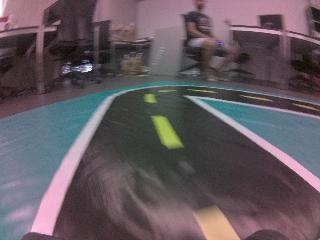
\includegraphics[height=0.50\textwidth]{experiments/11296.jpg}
  \end{minipage}%
  \begin{minipage}{.50\textwidth}
      \centering
      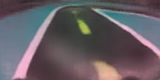
\includegraphics[width=0.60\textwidth]{experiments/11296.png}
  \end{minipage}
  \captionof{figure}{Real world image processed after cropping with a VAE, z\_size=64 and no augmentation. Reconstruction\_loss=112}
  \label{fig:realvaeexample}
\end{figure}
\begin{figure}
  \begin{minipage}{.50\textwidth}
    \centering
    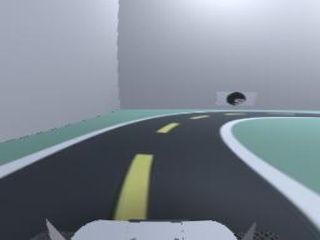
\includegraphics[height=0.50\textwidth]{experiments/1160.jpg}
  \end{minipage}%
  \begin{minipage}{.50\textwidth}
      \centering
      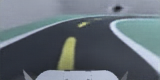
\includegraphics[width=0.60\textwidth]{experiments/1160.png}
  \end{minipage}
  \captionof{figure}{Simulator image processed after cropping with a VAE, z\_size=64 and no augmentation. Reconstruction\_loss=17}
  \label{fig:simvaeexample}
\end{figure}

\begin{table}
  \centering
  \begin{tabular}{|c|c||c|c|c|c|}
  \hline
  Z\_SIZE & AUGMENTATION & MEAN & STD & MAX & MIN \\ \hline
  \multirow{2}{*}{32} & False & 121.54 & 102.42 & 795.44 & 45.61 \\
  & True & 164.57 & 95.51 & 783.03 & 65.13  \\ \hline
  \multirow{2}{*}{64} & False & 103.54 & 79.14 & 588.14 & 40.84 \\
  & True & 137.24 & 74,02 & 611,81 & 63,05  \\ \hline
  \end{tabular}
  \caption{AE trained in simulation - reconstruction loss}
  \label{tab:aesim}

  \begin{tabular}{|c|c||c|c|c|c|}
  \hline
  Z\_SIZE & AUGMENTATION & MEAN & STD & MAX & MIN \\ \hline
  \multirow{2}{*}{32} & False & 377.07 & 87.53 & 756.7 & 239.46 \\
  & True & 493.84 & 99.40 & 807.67 & 289.99  \\ \hline
  \multirow{2}{*}{64} & False & 311.1 & 78.5 & 695.65 & 177.77 \\
  & True & 411.37 & 77.30 & 647.68 & 241.87 \\ \hline
  \end{tabular}
  \caption{AE trained in real world - reconstruction loss}
  \label{tab:aereal}

  \begin{tabular}{|c|c||c|c|c|c|}
  \hline
  Z\_SIZE & AUGMENTATION & MEAN & STD & MAX & MIN \\ \hline
  \multirow{2}{*}{32} & False & 59.1 & 60.41 & 620.93 & 18.88 \\
  & True & 116.31 & 71.11 & 771.88 & 51.10  \\ \hline
  \multirow{2}{*}{64} & False & 45.15 & 43.49 & 480.22 & 14.34 \\
  & True & 112.17 & 59.79 & 573.19 & 54.28  \\ \hline
  \end{tabular}
  \caption{VAE trained in simulation - reconstruction loss}
  \label{tab:vaesim}

  \begin{tabular}{|c|c||c|c|c|c|}
  \hline
  Z\_SIZE & AUGMENTATION & MEAN & STD & MAX & MIN \\ \hline
  \multirow{2}{*}{32} & False & 227.4 & 44.74 & 418.7 & 140.12 \\
  & True & 263.87 & 52.29 & 478.26 & 172.70 \\ \hline
  \multirow{2}{*}{64} & False & 184.56 & 36.86 & 347.59 & 96.7 \\
  & True & 230.66 & 42.24 & 402.67 & 156.61  \\ \hline
  \end{tabular}
  \caption{VAE trained in real world - reconstruction loss}
  \label{tab:vaereal}
\end{table}


\begin{center}
    \begin{minipage}{0.9\linewidth}
      \lstinputlisting[caption=AE network, label=lst:aenet]{ae.txt}
      \end{minipage}
    \begin{minipage}{0.9\linewidth}
      \lstinputlisting[caption=VAE network, label=lst:vaenet]{vae.txt}
      \end{minipage}
\end{center}

\section{RL algorithm}

\subsection{Reward function}
Designing a reward function that can work on both simulated and real environments is not trivial. In simulation, the environment can provide a better supervision than a human can do. In our real setup we have only the camera frames as states and so no other sensor is available, even though they can be used. In simulation, instead, the environment can tell us how far the donkeycar is from the center line of the track, with this value, we can decrease the reward function by a value proportional to the distance of the car from the center of the roadway as done in Equation \ref{eq:stdreward}. So the reward function is:

\begin{equation}
  \label{eq:stdreward}
    r_t = 1 + throttle\_reward + cte\_penalty + \left\{\begin{matrix}
    if done & crash\_error \\ 
    else & 0  
    \end{matrix}\right.
\end{equation}
where 1 is given for each step taken by the agent in order to incentivize the completion of the largest possible number of steps. The throttle reward incentives the car to go as fast as possible, however in our setup, the throttle is kept constant for the purposes of this thesis. The Cross Track Error (CTE) penalty, is a negative value to incentive the car to stay as close as possibile to the center of the roadway. In case the car exceeds a predefined maximum CTE or crashes, the penalty becomes very high and it is added through the \textit{crash\_error} term. 
This first reward function is used to test our algorithm and after proving it can work, we need to adapt it such that it can work also in real world. To tackle the issue we simply remove the CTE penalty with a negative value to be activated only when an episode ends due to human intervention. The final reward function that has proven to work in both environment and we use in our trainings is:
\begin{equation}
  \label{eq:realreward}
    r_t = 1 + throttle\_reward + \left\{\begin{matrix}
    if done & crash\_error \\ 
    else & 0  
    \end{matrix}\right.
\end{equation}
Since we want the real and the simulated version of our agent as similar as possibile Equation \ref{eq:realreward} is used in both cases.

\subsection{Training the simulated RL agent}
As a baseline for RL algorithm we used the source code provided by \citet{DBLP:journals/corr/abs-2008-00715}. Their algorithm allows both simulated and real training, however training on simulation with communication being over-the-internet is more computationally expensive and more prone to errors. Thus, for the simulation, we refactor the algorithm such that the communication happens locally. Beside that, his algorithm uses an AE which need to be changed with the VAE chosen above. Given that the simulator provides several training modality we test them all to find out which one is the best, to eventually save time in real world. To chose where the car should starts a new lap we trained 4 different model, one for each option provided by the simulator, to identify which one eventually converges and if it does. The quality measures, illustrated below in Figure \ref{fig:agentresults}, are the \textit{Episode success rate} that shows how many laps has been complete on average, the \textit{Episode Reward mean} and the \textit{Episode Length mean}. All the model have been trained for 100k iterations, with a different starting point.\textit{ Agent 1} started each lap at a random checkpoint,\textit{ Agent 2} started always at the starting line,\textit{ Agent 3} at the latest checkpoint reached during the last episode and, finally,\textit{ Agent 4} cyclically uses all the checkpoints.
\begin{figure}[h]
  \centering
  \begin{subfigure}{.5\linewidth}
      \centering
      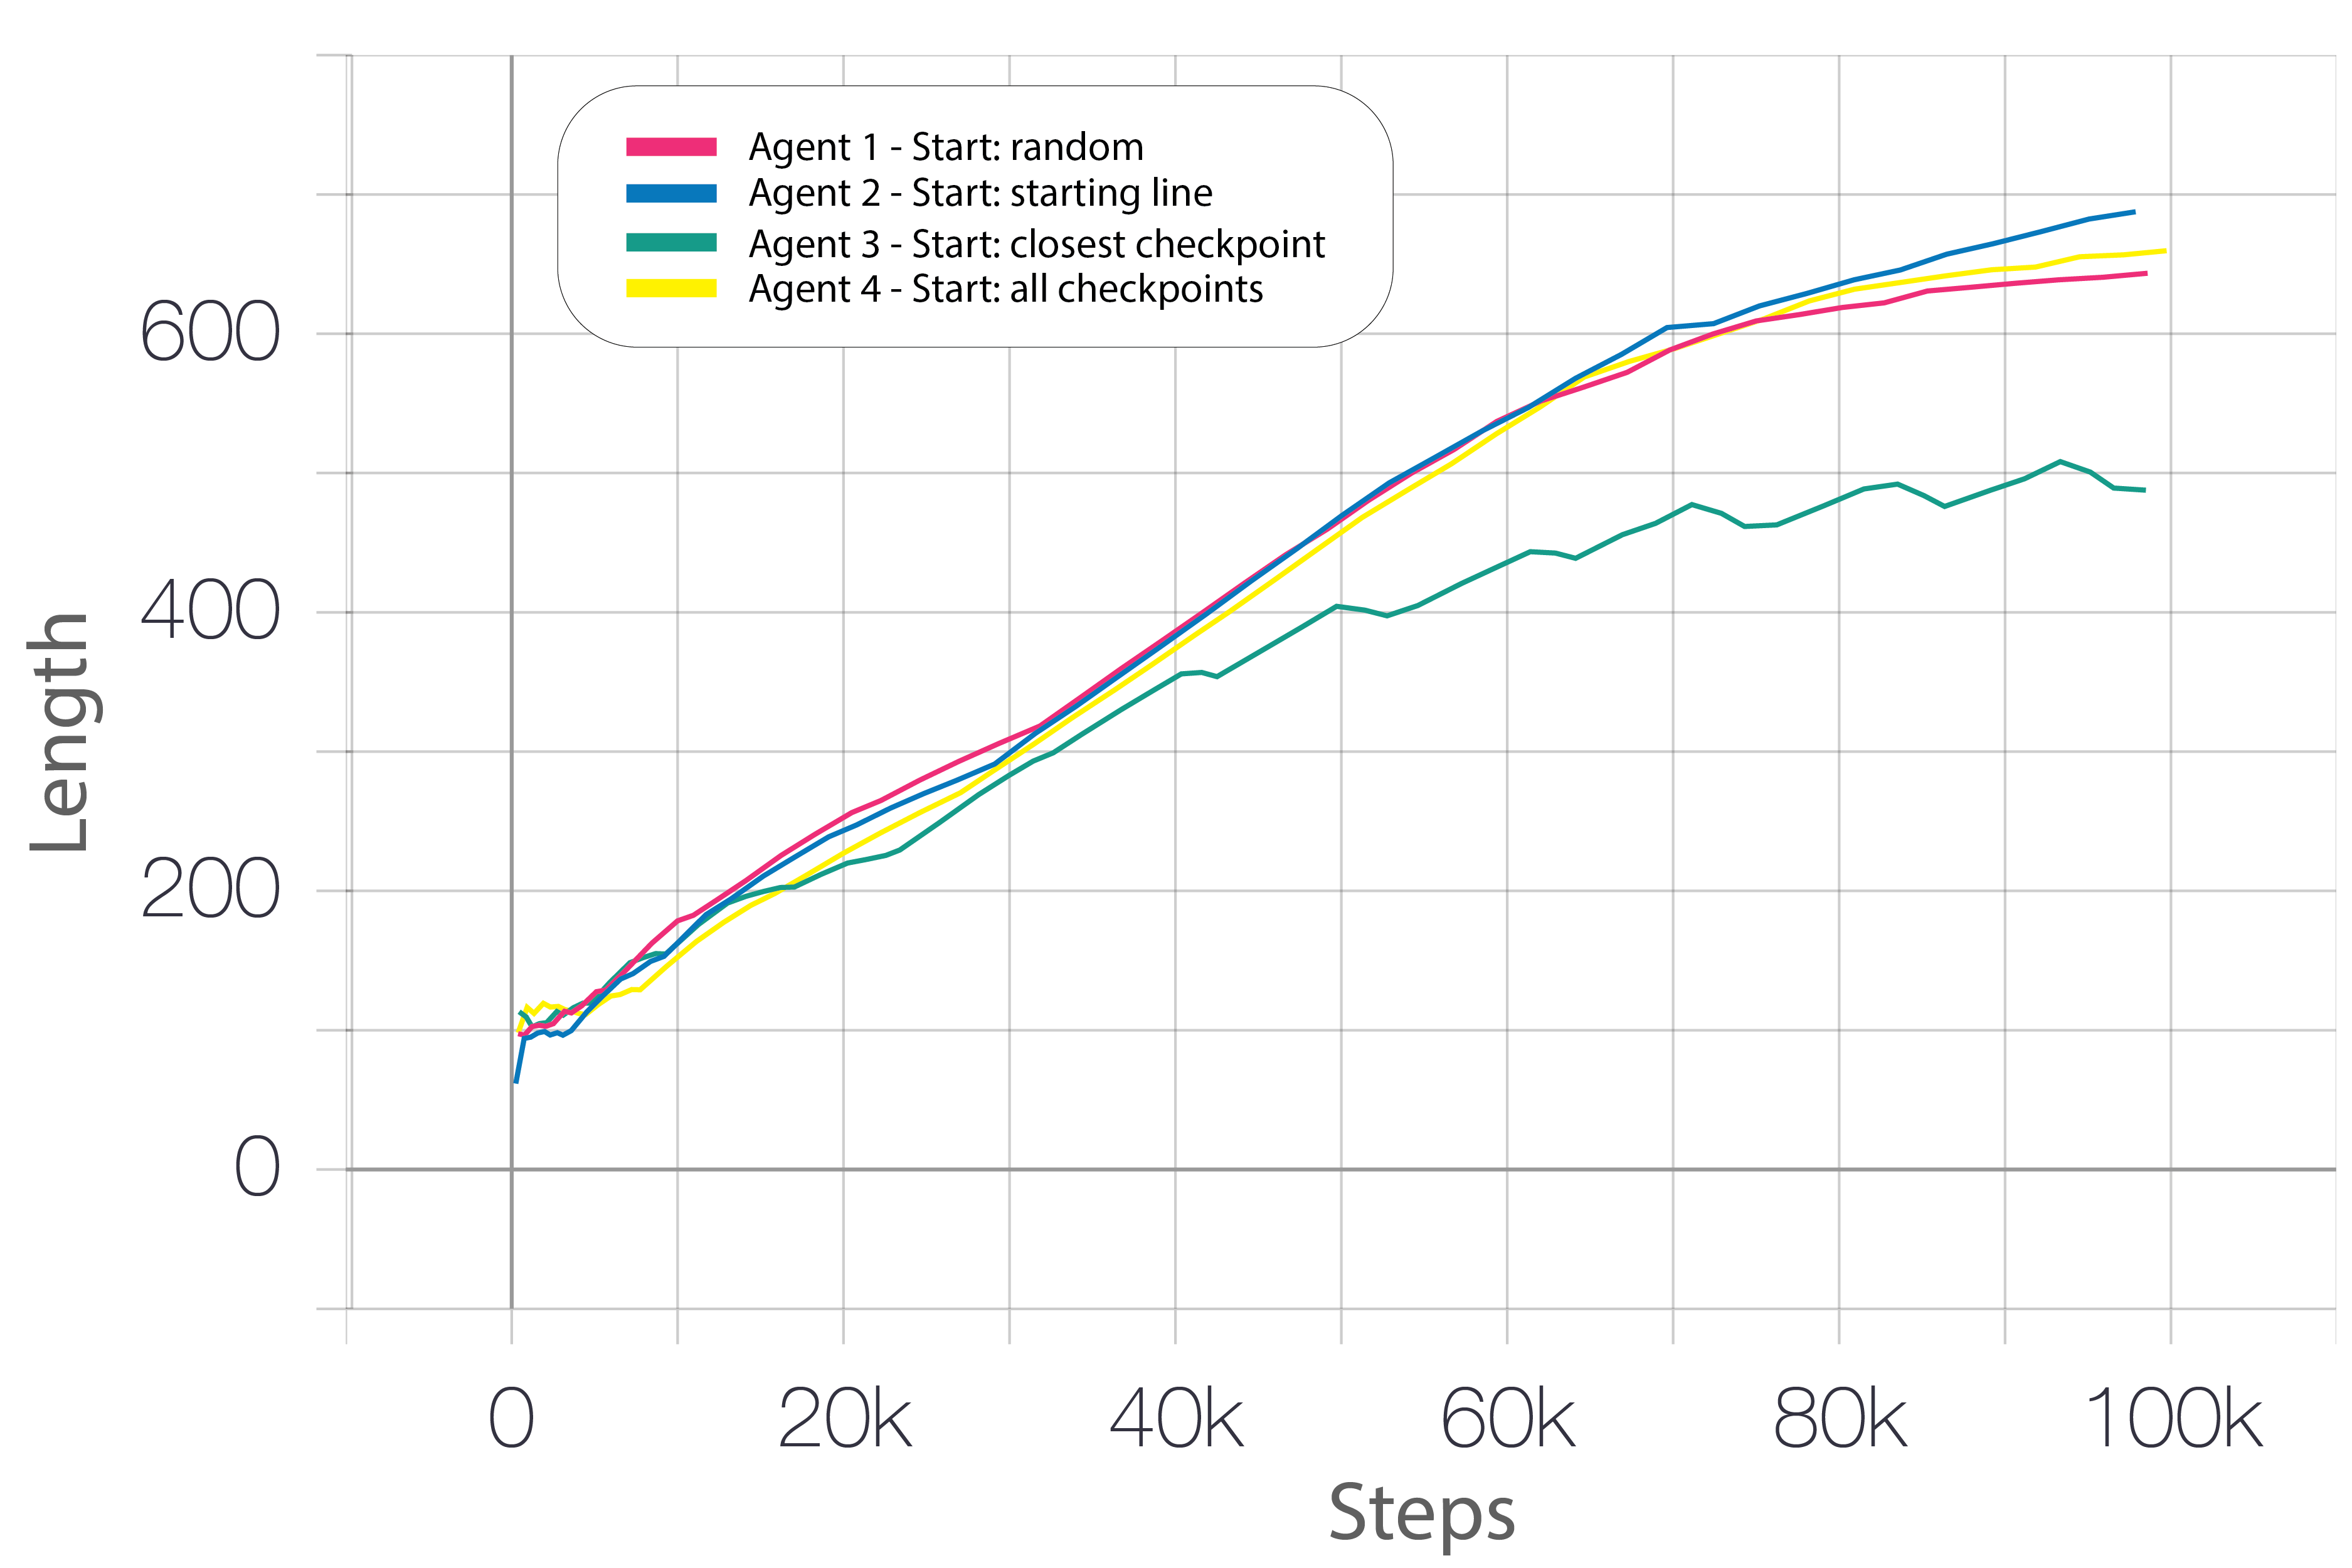
\includegraphics[width=1\textwidth]{experiments/len_mean.png}
      \caption{Episodes length mean}\label{fig:len}
  \end{subfigure}%
      \hfill
  \begin{subfigure}{.5\linewidth}
      \centering
      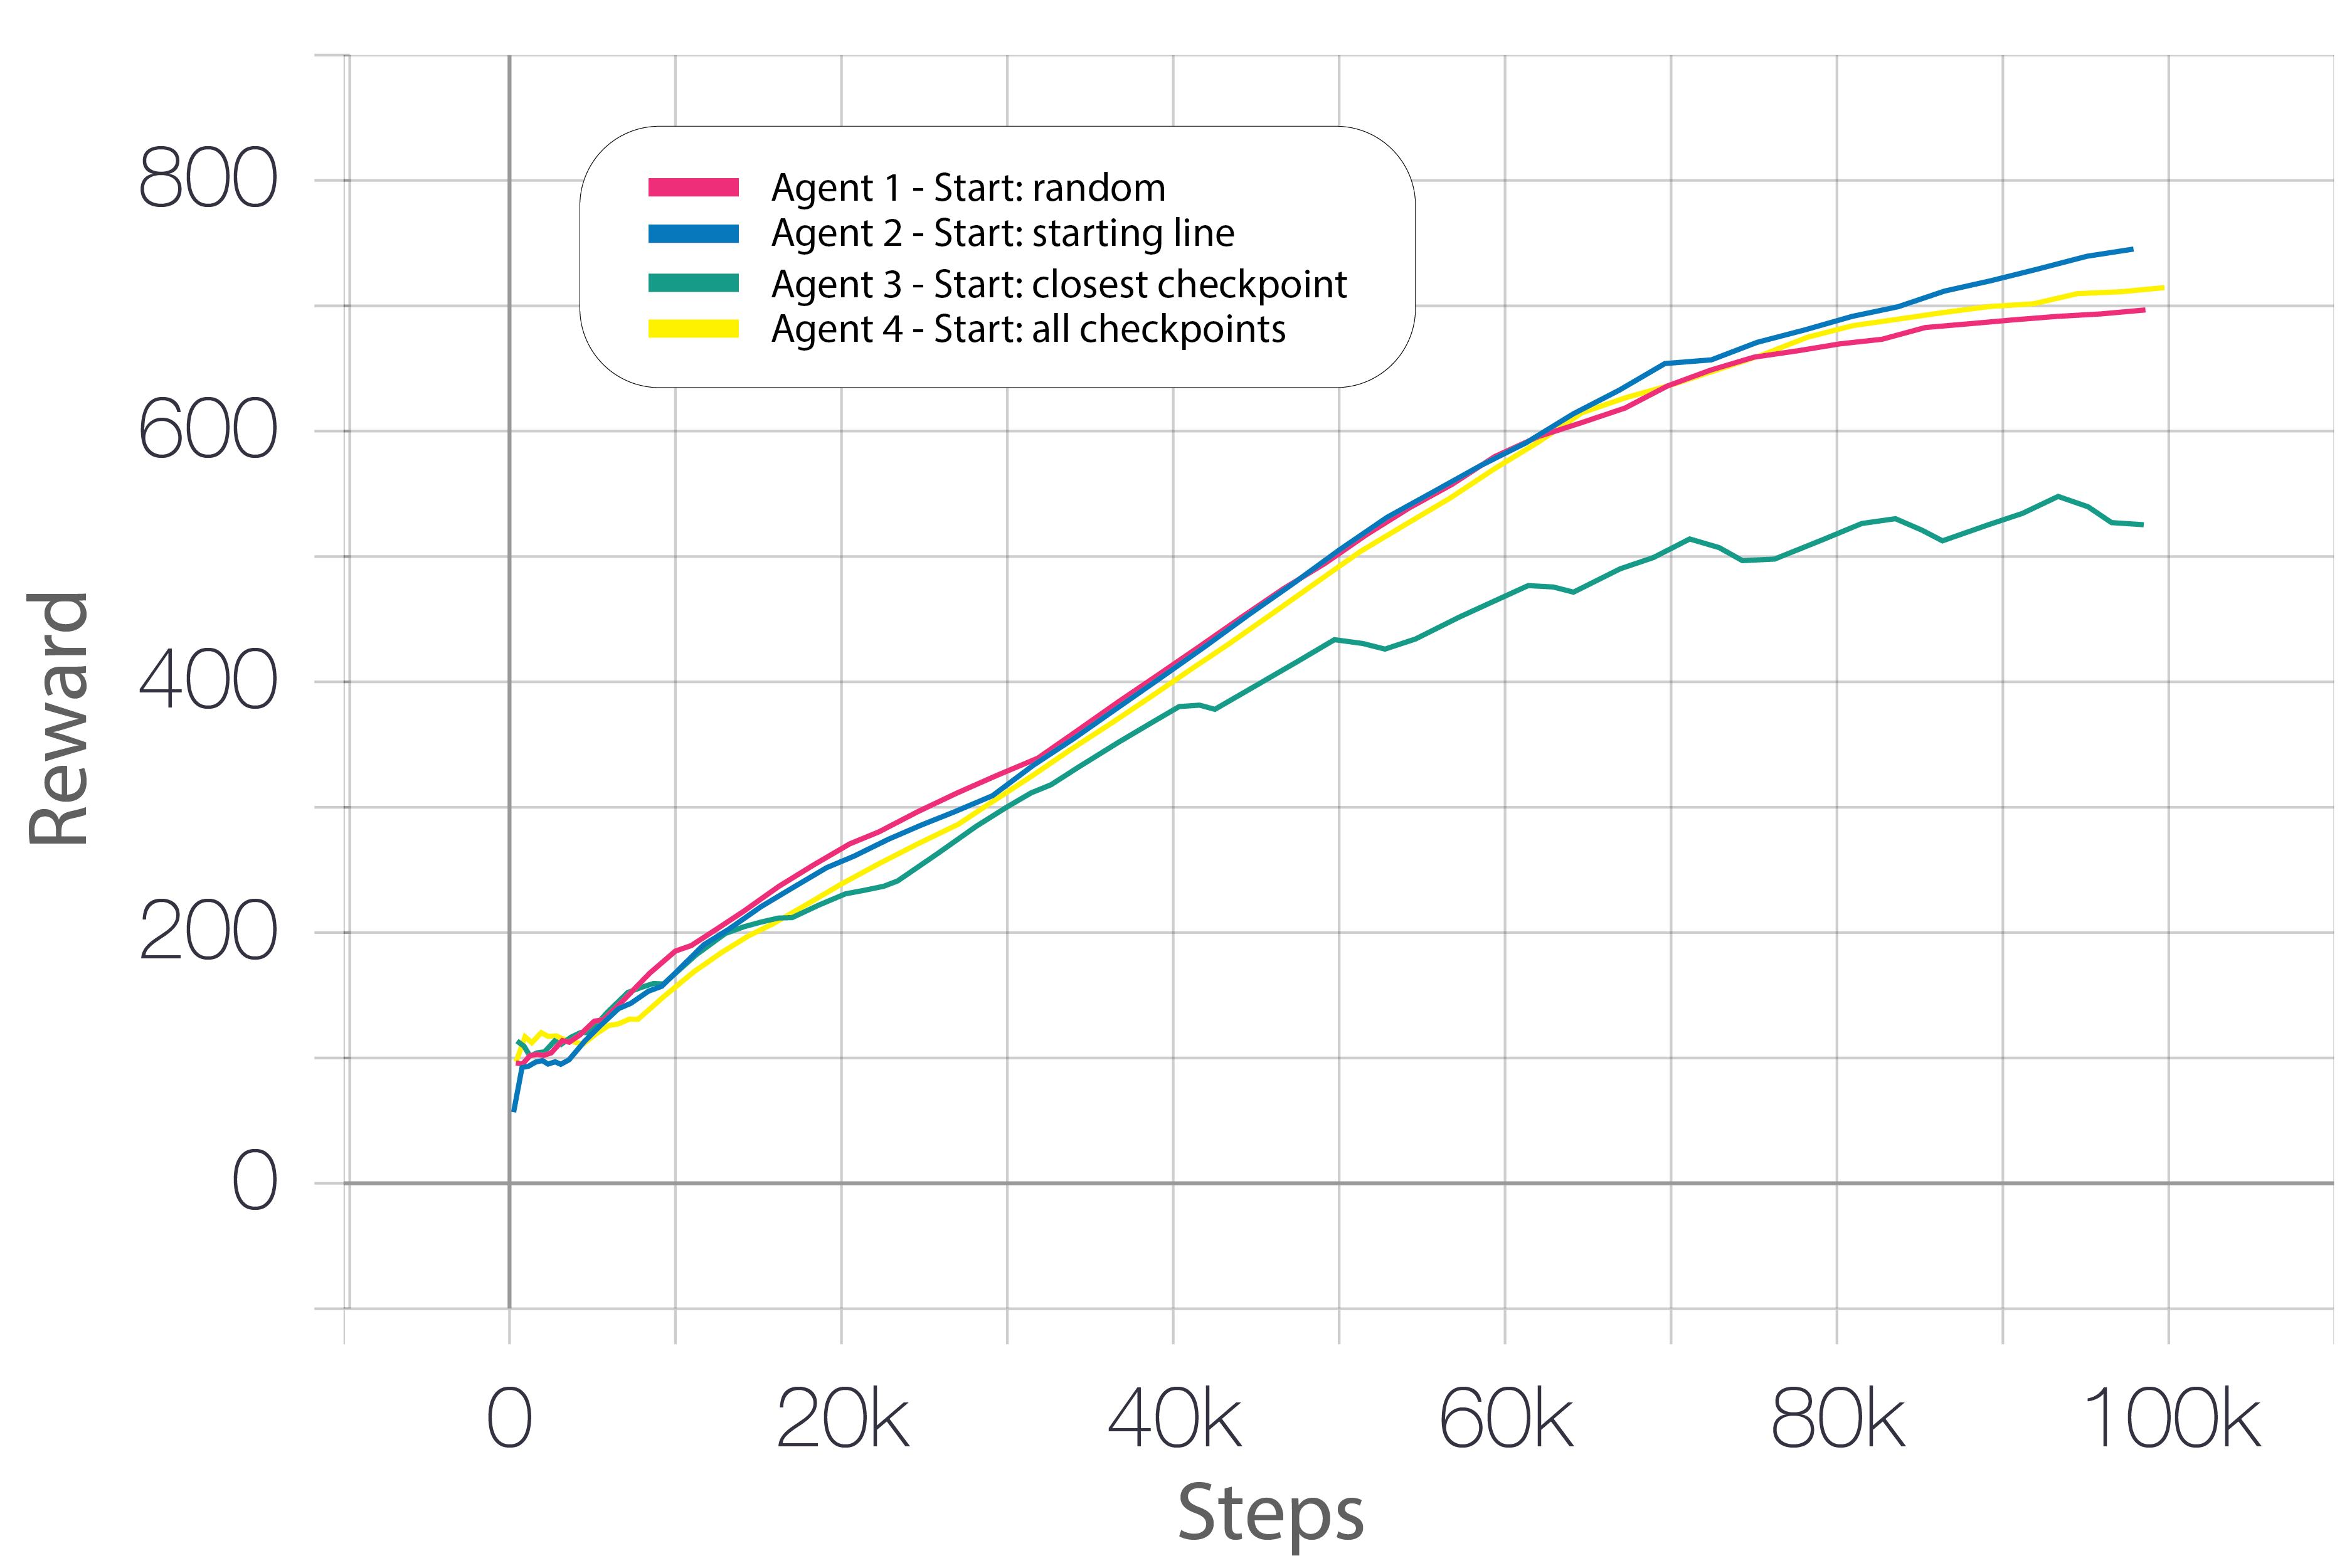
\includegraphics[width=1\textwidth]{experiments/rew_mean.png}
      \caption{Episodes reward mean}\label{fig:rew}
  \end{subfigure}
  
  \bigskip
  \begin{subfigure}{.5\linewidth}
    \centering
    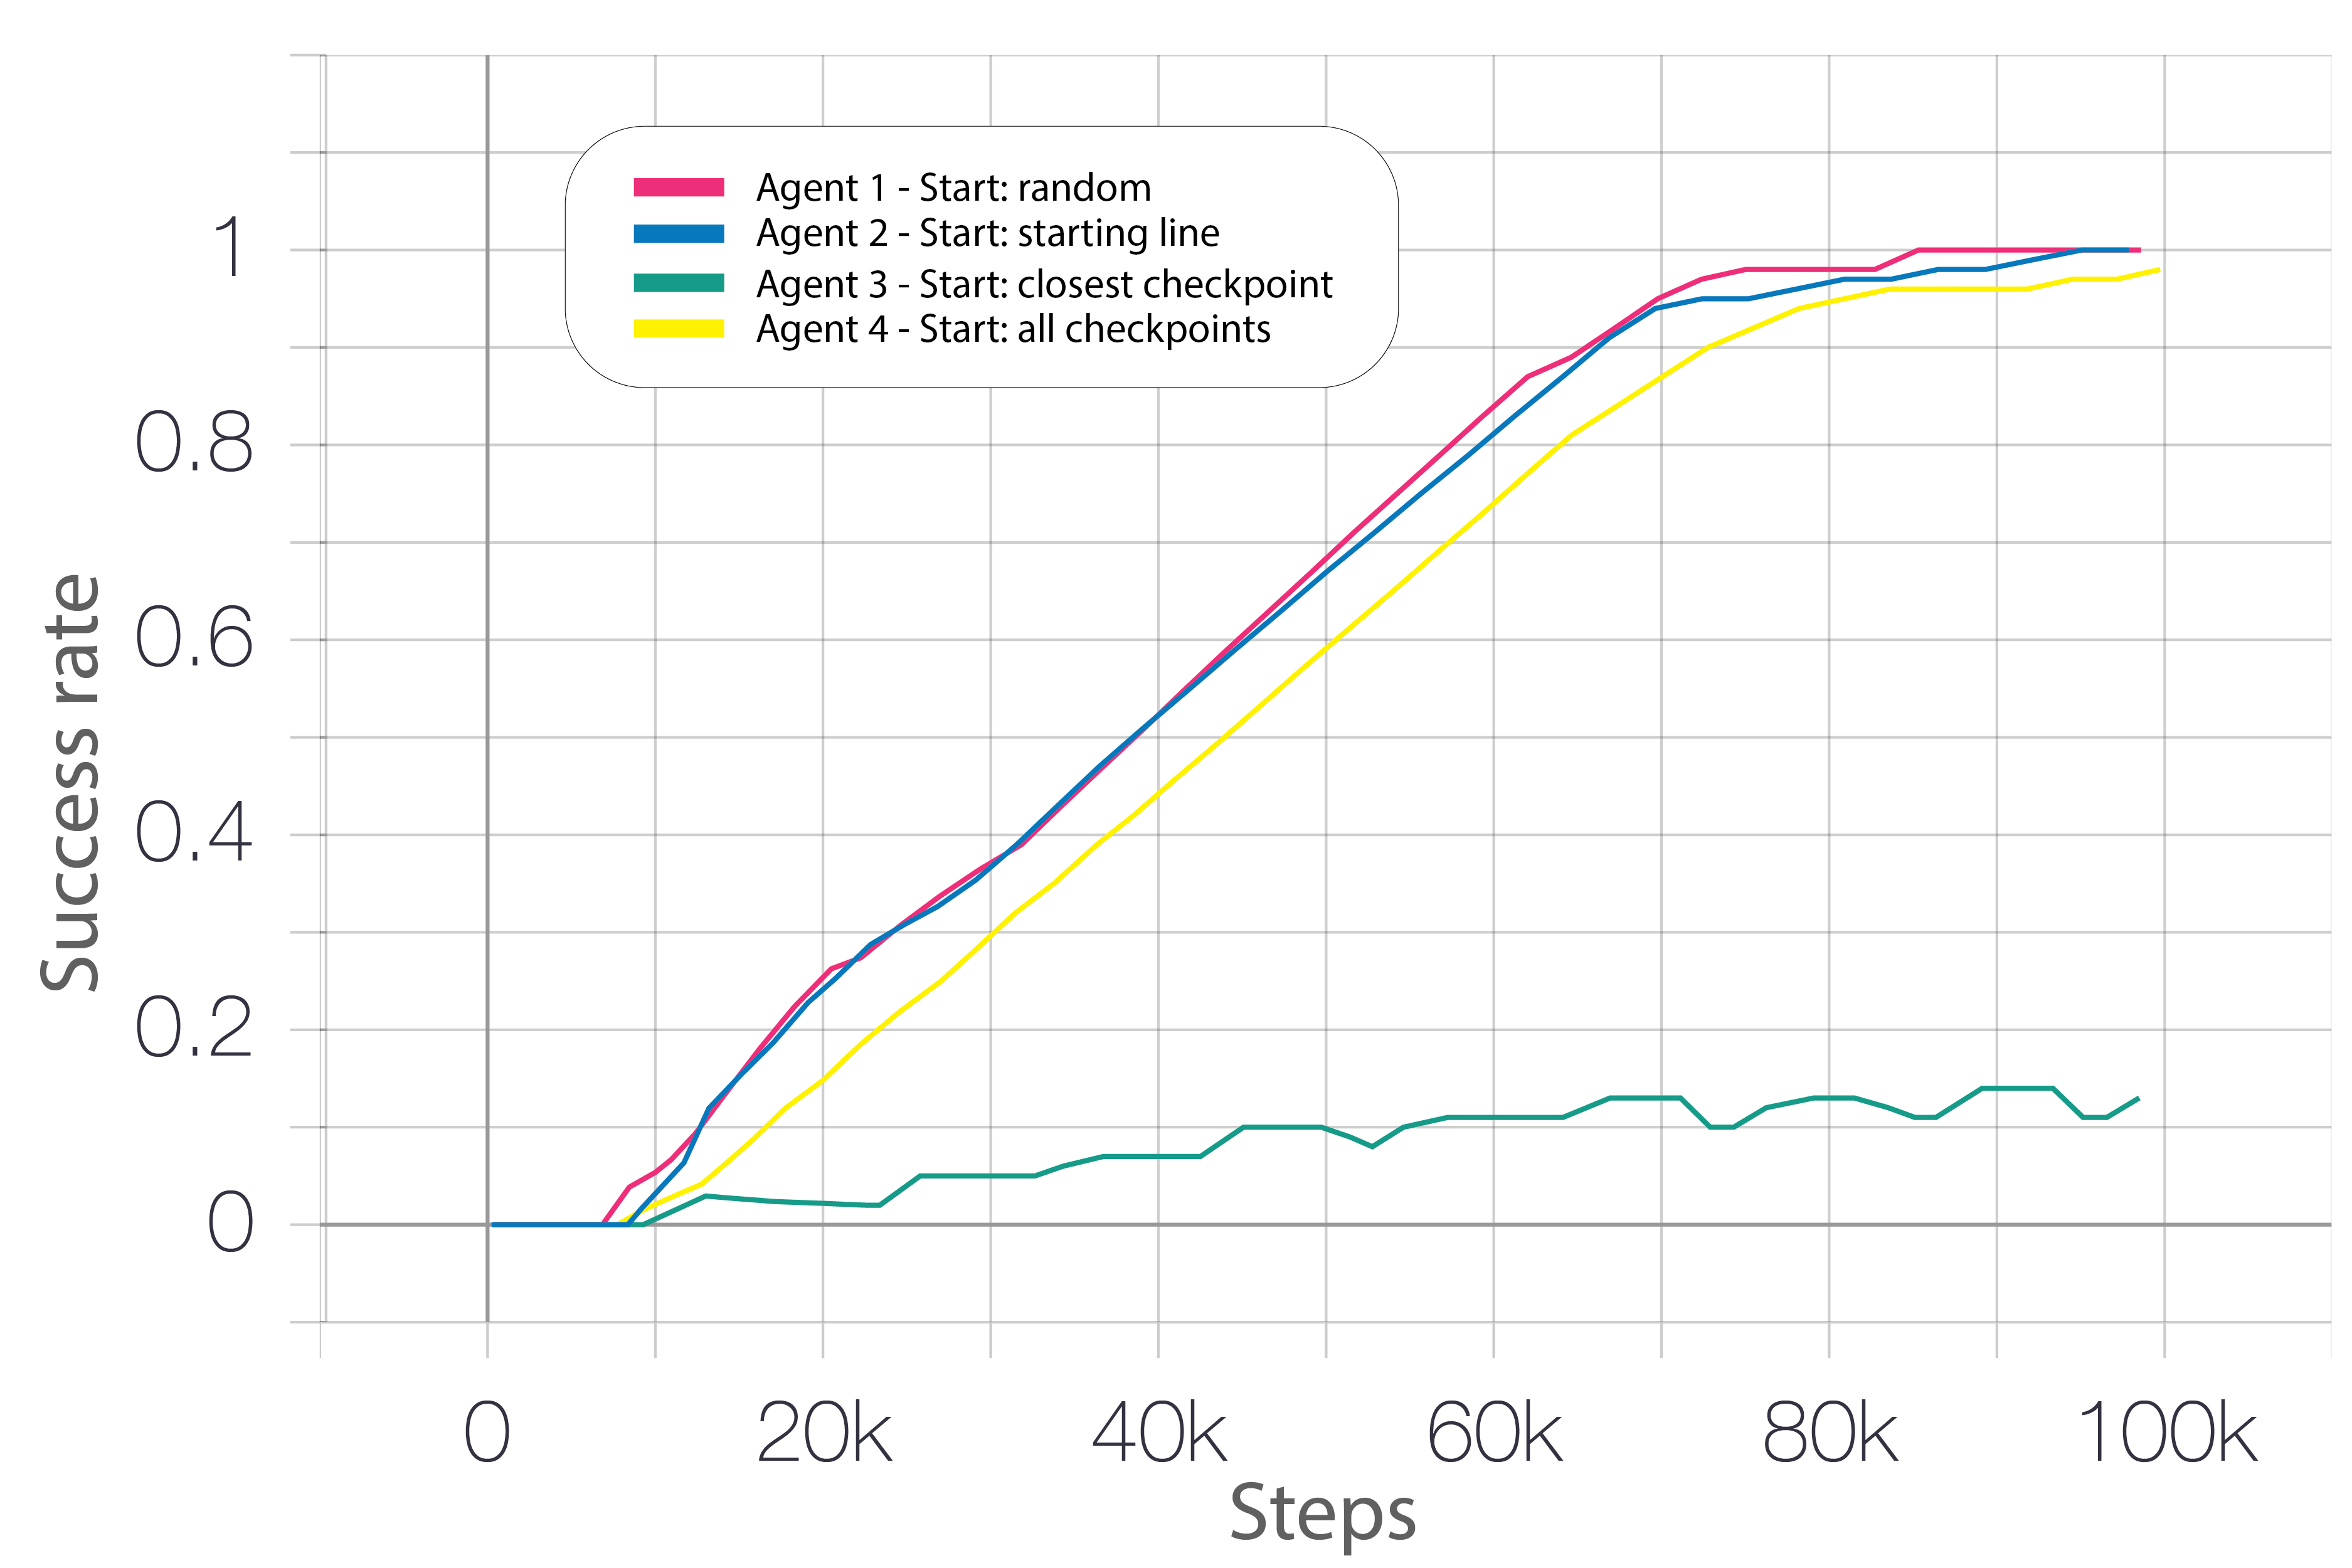
\includegraphics[width=1\textwidth]{experiments/success_mean.png}
    \caption{Success rate mean}\label{fig:succ}
  \end{subfigure} 
  \caption{Agents trained in simulation. Each agent has been trained with a different starting modality and has been trained for 100k steps.}
  \label{fig:agentresults}
\end{figure}
During our experiments we noted that, in the best case, a lap may takes $\sim 350$ iterations to be completed. Our agents are all able to successfully learn to drive with a strict maximum CTE except for the agent that started new laps from the latest checkpoint. There are two interesting evidences that come out of those trainings. The first one is that even though the success rate mean approaches $100\%$, that means the agent is able to consistently finish laps, the reward mean keeps growing. This shows a limitation in the reward function used, given that the agent gets a reward for every steps, it learns to finish the lap following the longest path it has discovered. Beside that, the best way to lengthen the path is a zig-zag behavior that allows also a doubling of the reward per lap. Secondly, the agent that start at the latest checkpoint keeps improving the reward up to more than an equivalent completed lap, however it never finishes a lap as described in Figure \ref{fig:succ}. The reason behind this strange behavior is that the agent found a bug in the simulator used, as shown in Figure \ref{fig:bug}. Essentially, there is a a little spot, off track, close to the steepest turn where the CTE is not is correctly detected and consequently the episode is not terminated. The fact this behavior happens only on this agent stands in the training modality. When the agent reach this checkpoint, he cannot easily reach the next checkpoint given the toughness of the turn, instead it finds much easier to explore the bugged spot which is almost right in front of it when it approaches the turn.

\begin{figure}[h]
  \begin{center}
    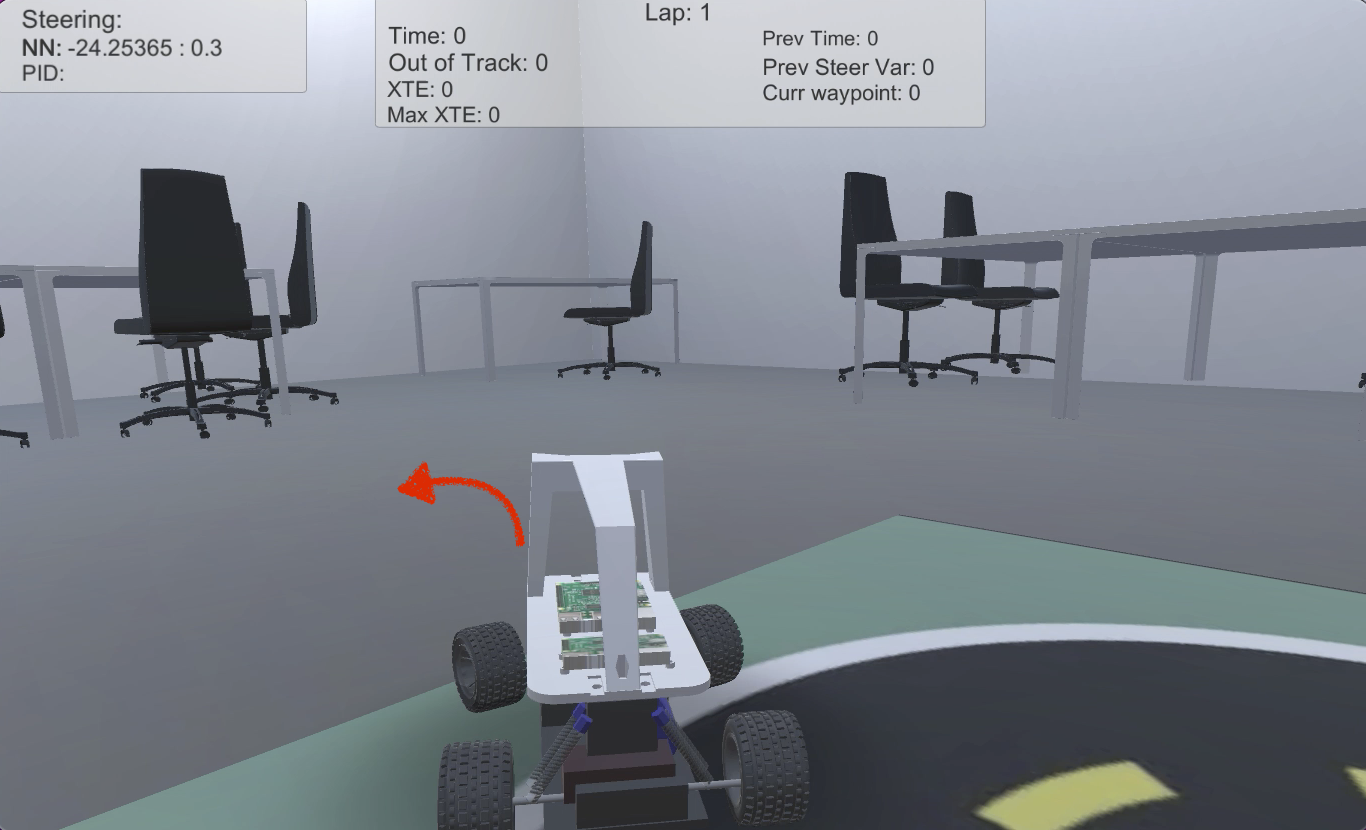
\includegraphics[width=0.50\textwidth]{experiments/bug.png}
  \end{center}
  \caption{Spotted bug in the simulator}
  \label{fig:bug}
\end{figure}

To furter test the trained agents, for 10 laps it is measured how many times the lap has been completed, how many times the agents crashes, and finally after disabling the CTE threshold, if the agent is still able to recover and finish the lap without crashing. The result are presented in Table \ref{tab:simagent}.

\begin{table}
  \centering
  \begin{tabular}{|c|c|c|c|c|c|}
  \hline
  AGENT & OOT & OBE & LAPS & AVG LENGTH & AVG REW \\ \hline
  1 & 0 & 0 & 10 & 595 & 644 \\
  2 & 0 & 4 & 10 & 599 & 647  \\ \hline
  3 & 0 & 0 & 10 & 624 & 676 \\
  4 & 10 & 29 & 0 & 460 & 495  \\ \hline
  \end{tabular}
  \caption{Agents results averaged over 10 laps. Out Of Track (OOT) measures crashes, Out of Bound Error measure how many times it exceed the max CTE, and finally LAPS counts the completed laps.}
  \label{tab:simagent}
\end{table}

Thus, excluding\textit{ Agent 4 }because of the simulator's bug, three agents learned to drive successfully and in most cases they always stay entirely on track without the need of any additional sensor and with the only problem of the shaky driving which is still acceptable for the purposes of this thesis.

\subsection{Training the real RL agent}
In real world instead the source code provided by \citet{DBLP:journals/corr/abs-2008-00715} is kept untouched beside the encoder, with the main goal being to replicate their results but with a more performing VAE as resulted in our tests. Given that in real world the simulator supervision is not available, all the agents tested in previous section are good candidates to be used, also \textit{Agent 4} that cannot explore anymore the simulator's bug. However from the tests, it resulted that all the agents struggle to learn driving an entire lap in reasonable time, except\textit{ Agent 4 }that start his laps at the latest checkpoint reached in the last episode. Human supervision is about stopping the episode anytime the car exceeds the track boundaries with all 4 wheels, while the host machine automatically stops the car when it reaches 1000 steps ($\sim 2.5$ laps). In figure \ref{fig:realresult} are shown the performances in training. The laying of the car on the latest checkpoint has been intentionally approximate on the area close to the checkpoint. This brought a main advantage, the agent learns quicker since it is able to see the area in front of it from many points of view. It results useful when the car will start to cross many checkpoints per episode, since the direction from which the car arrives to a checkpoint can vary a lot, it has been trained to drive on many possibile trajectories and will join the various sections well. The overall training procedure results to be simple and fast ($\sim$ 30 minutes) to get an entire lap completed. In five to twenty episodes, the first two turn are learned decently. Most of the time is spent on the steepest turn. As shown in Figure \ref{fig:rlen}, the graph is characterized by ups and downs, as soon as the car starts at the starting line, it learns quickly, then, when the steepest curve is reached it struggle to overcome it and the when it enventually does the length start to increase again. The process is repeated until it is almost consistently able to finish a lap. As soon as the agent has learned the steepest turn, it generalizes well on following turn, in fact little time is spent on them.

\begin{figure}[h]
  \centering
  \begin{subfigure}{.5\linewidth}
      \centering
      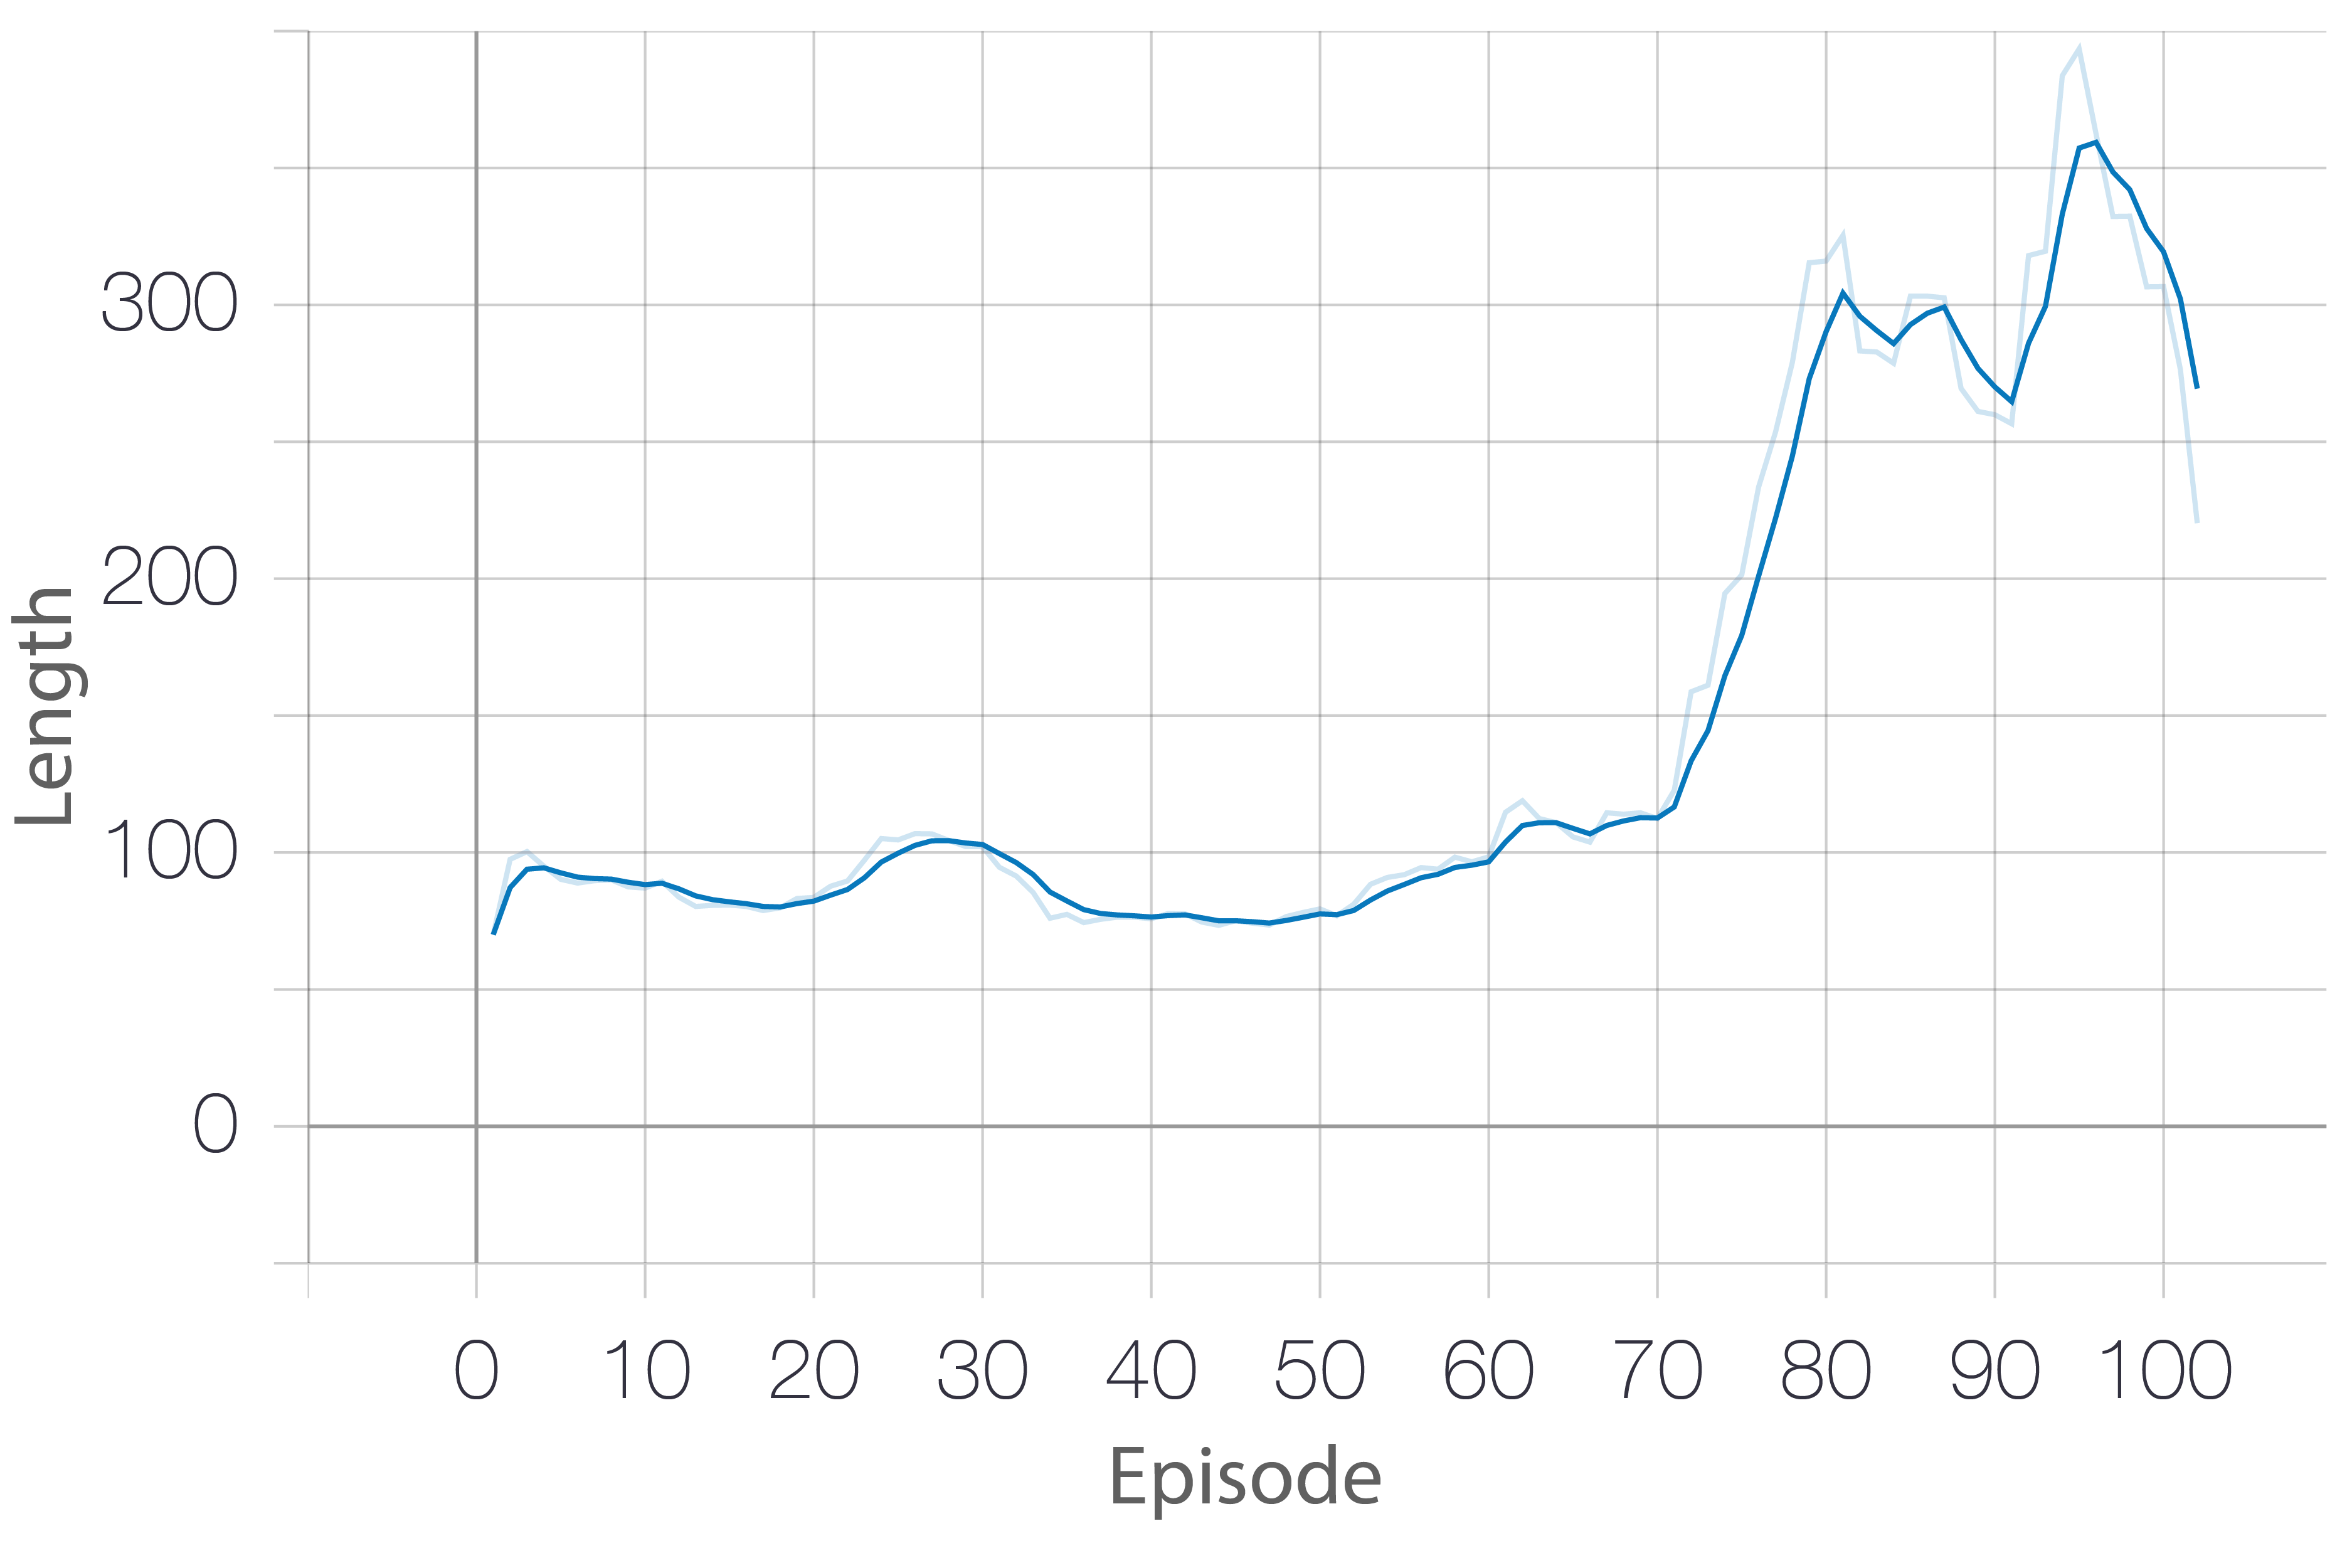
\includegraphics[width=1\textwidth]{experiments/real_len.png}
      \caption{Episodes length}\label{fig:rlen}
  \end{subfigure}%
      \hfill
  \begin{subfigure}{.5\linewidth}
      \centering
      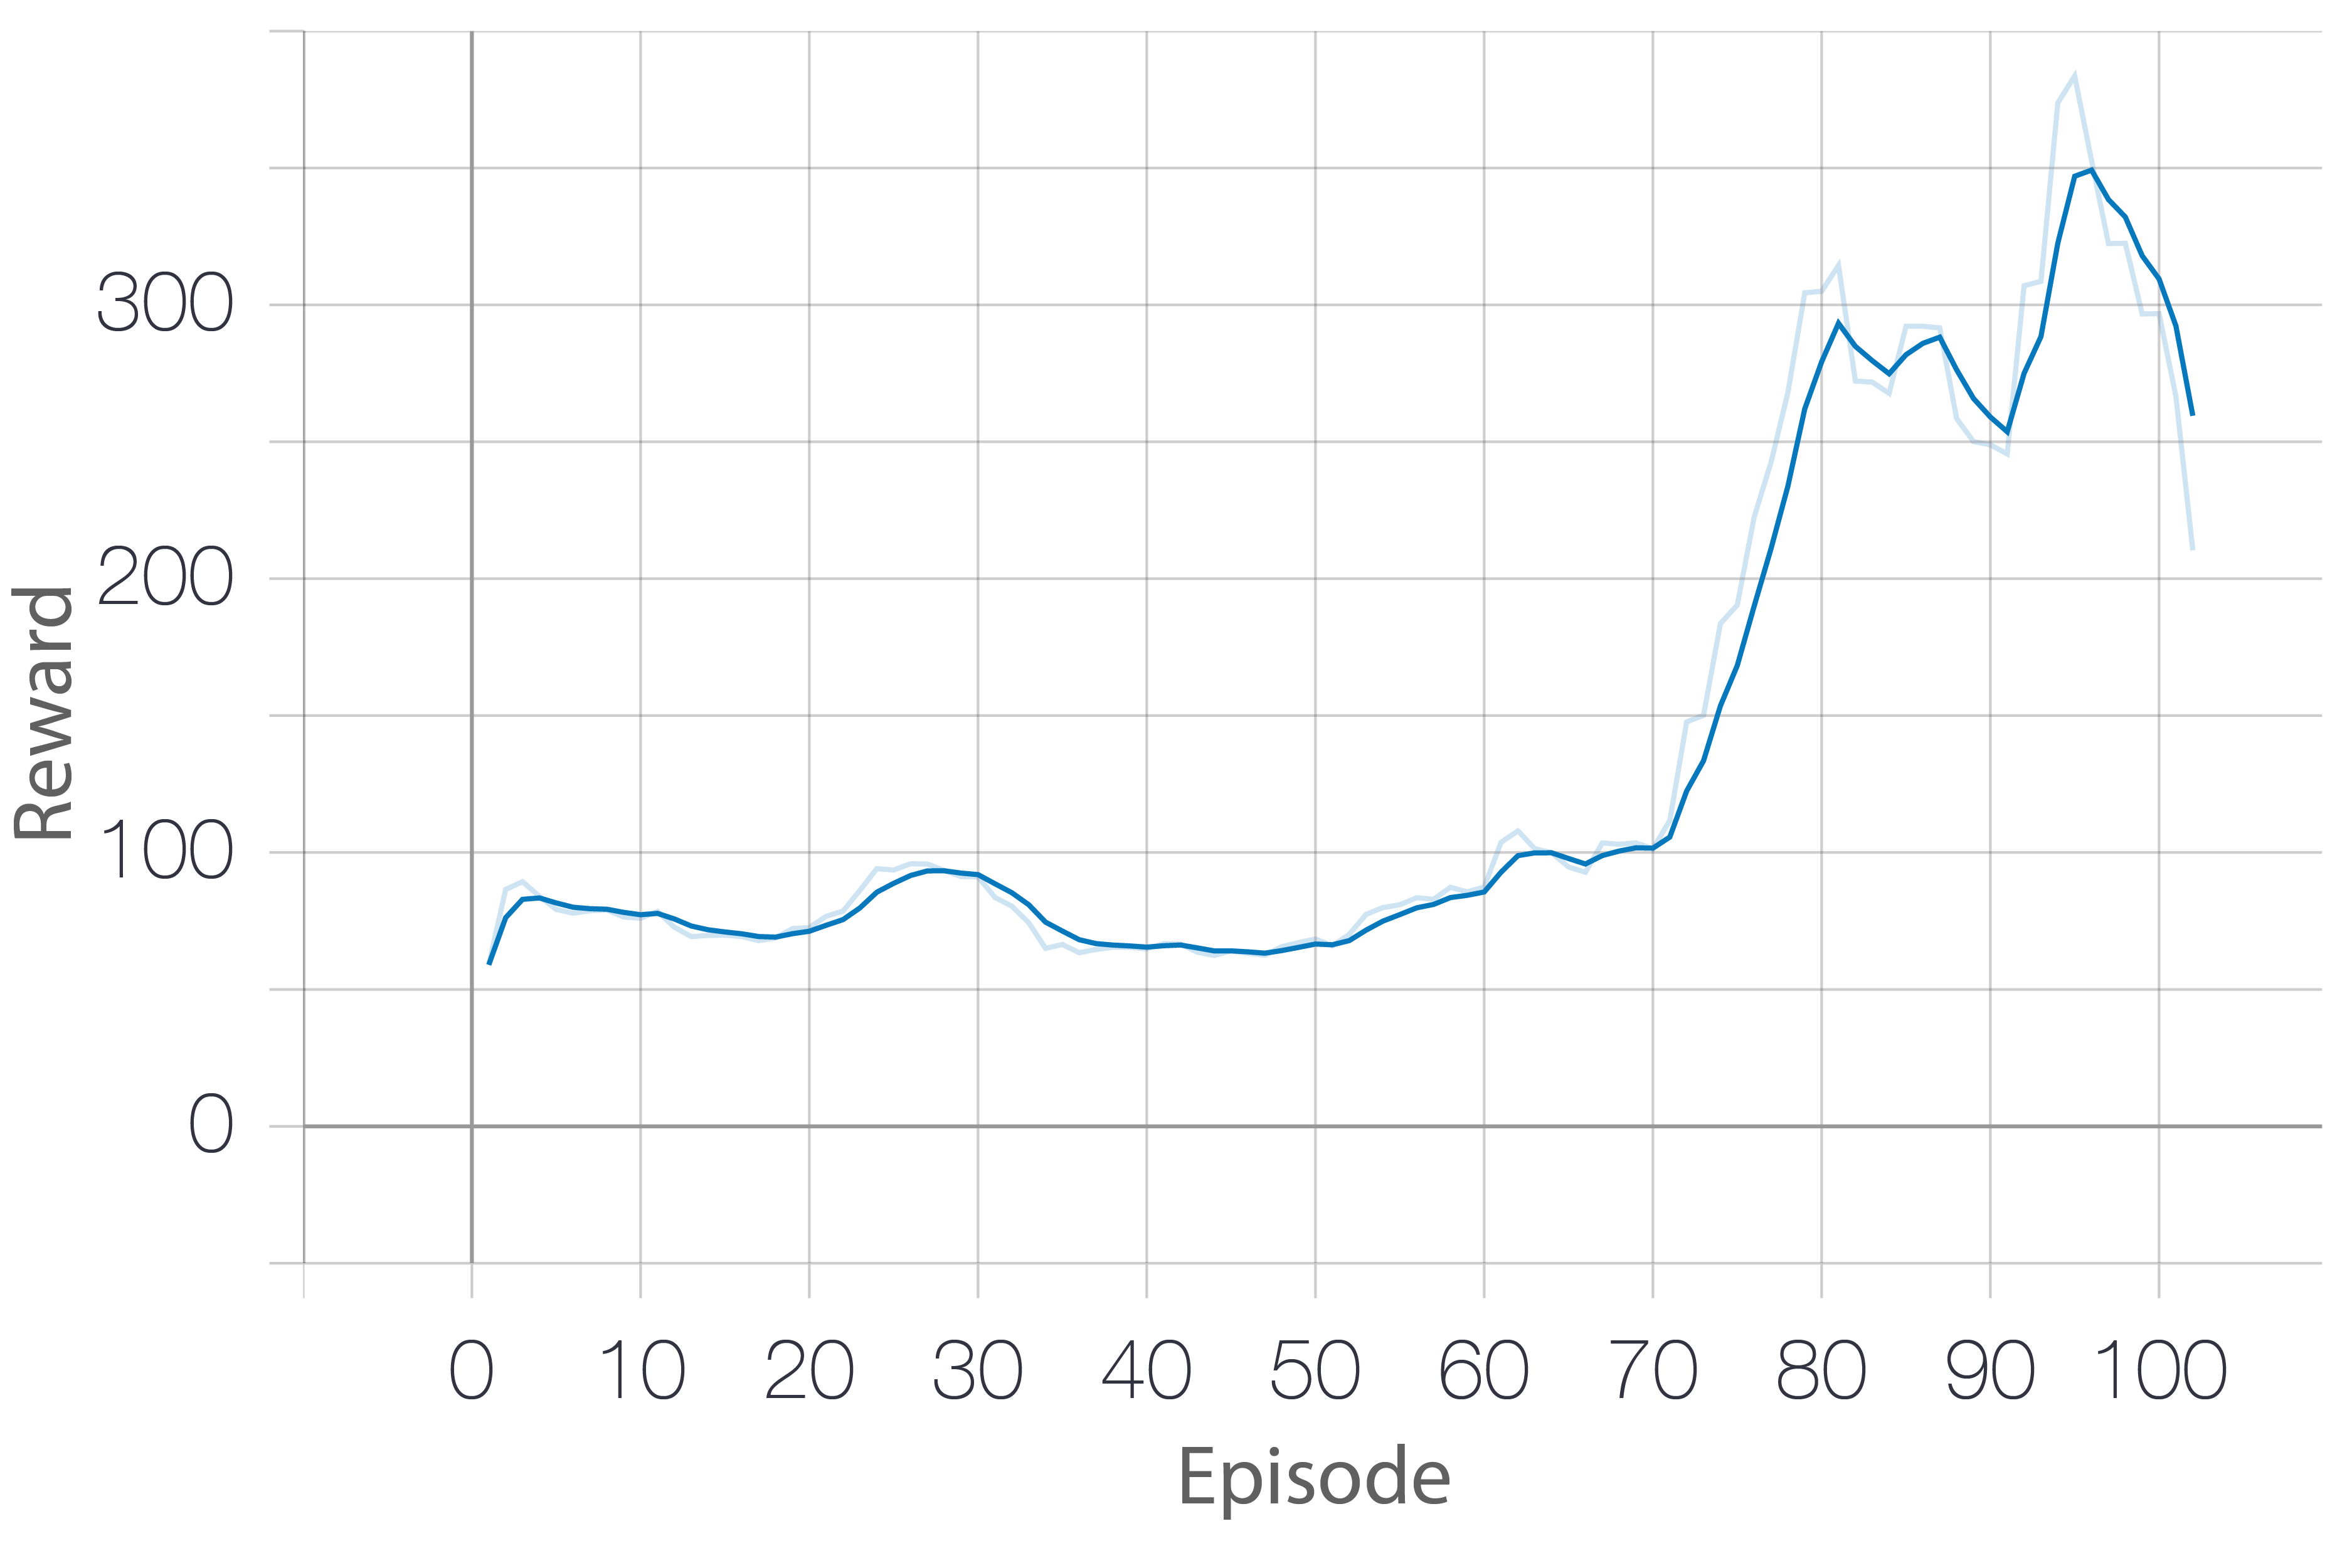
\includegraphics[width=1\textwidth]{experiments/real_rew.png}
      \caption{Episodes reward}\label{fig:rrew}
  \end{subfigure}
  \caption{Agent trained in real world starting each lap on the latest checkpoint}
  \label{fig:realresult}
\end{figure}

Unfortunately, in real world more metrics to measure the quality of the driving and to make comparisons with the simulated agents are not available. 

\section{Sim to Real}

SimToReal (S2R) or viceversa aims in deploying model trained in one environment to the other. In our case, since the real world environment, in our setup, does not provide enough metrics to benchmark our real world agents, we aim to make it works also in simulation. Another advantage brought by this approach is that an agent trained in simulation, can be moved into the real world and this would result in less expensive training procedures. The idea is to pre-train a CycleGan \citep{CycleGAN2017} for image trasfiguration. In fact, the CycleGan is able to move an image into another domain keeping the original structure unaltered, but applying the style of the other domain. Thus we leverage this property to transform images seen by the simulated camera of the DonkeyCar into what it would see in real world or viceversa. Then, a real agent will eventually be able to drive on the simulator since it does see pseudo-real images. On the other hand, in order to drive a real car with a simulated agent, our DonkeyCar has not enough computational power, hence it could not run in time a CycleGan, that has millions of parameters, in order to make the real car see pseudo-simulated images and drive with the simulated agent. However, the problem can be circumvented by training an agent entirely on simulation but with pseudo-real images.